\section{Testing \& Continuous Integration}
\label{sec:testing}

Quality and compatibility of the \apsq framework is ensured by a elaborate continuous integration (CI) which builds and tests the software on all supported platforms.
The CI structure and the different tests performed are detailed in the following.

\subsection{Continuous Integration}
\label{sec:ci}

\begin{figure}[btp]
  \centering
  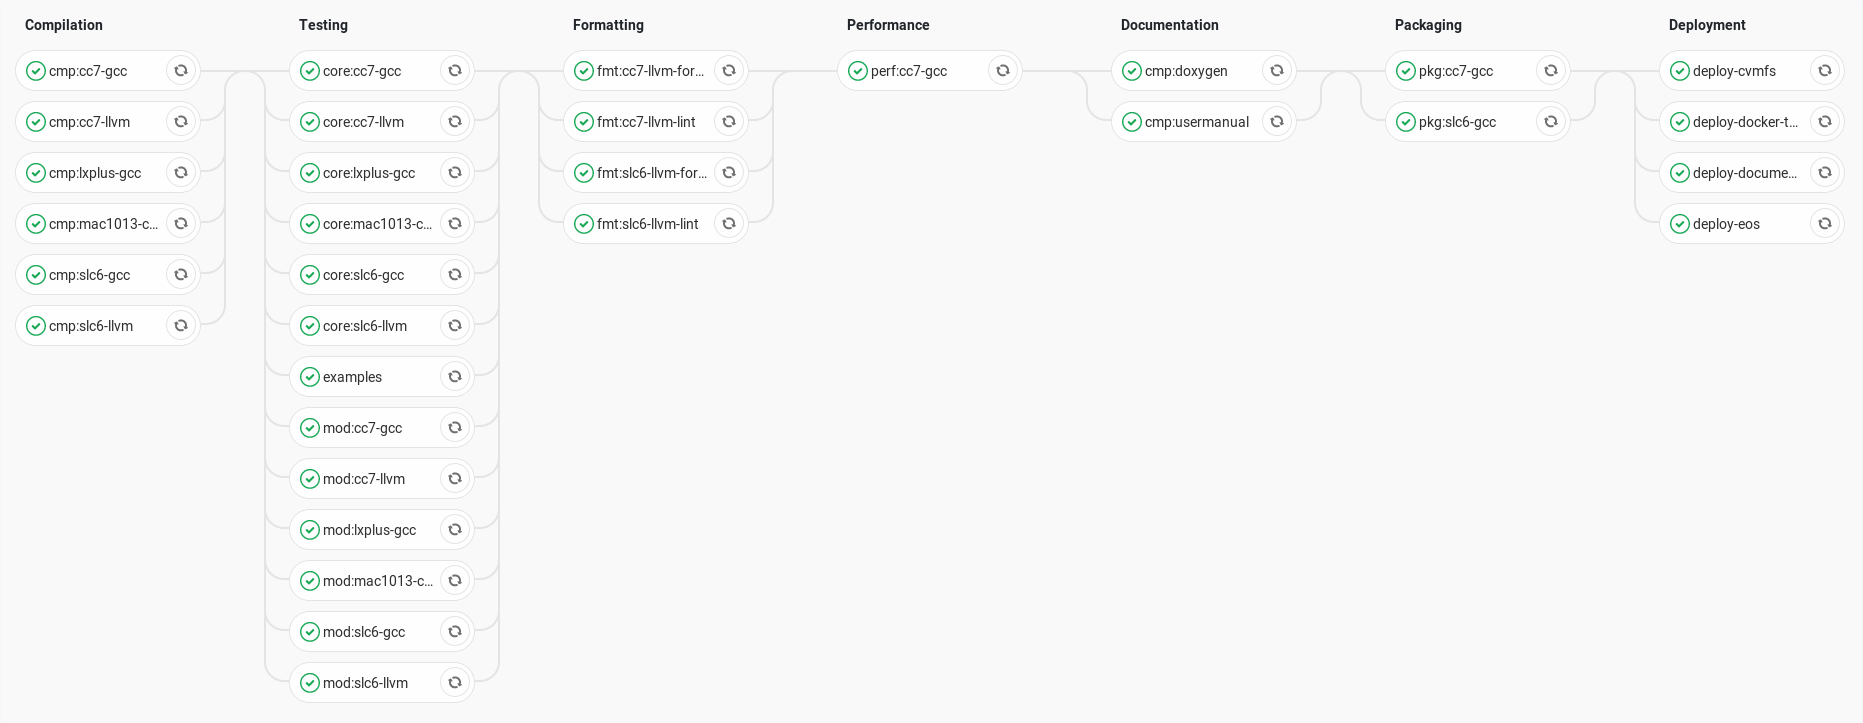
\includegraphics[width=\textwidth]{ci.png}
  \caption{Typical \apsq continous integration pipeline with 20 jobs distributed over five distinct stages. In this example, all jobs passed.}
  \label{fig:ci}
\end{figure}

The \apsq CI uses the integrated GitLab Continuous Integration and consists of five distinct stages.

The \textbf{compilation} stage builds the framework from the source on different platforms.
Currently, builds are performed on Scientifc Linux 6, CentOS7, and Mac OS X.
On Linux type platforms, the framework is compiled with GCC 7.1 and Clang 4.0, while AppleClang 8.1 is used on Mac OS X.
The build is always performed with the default compiler flags enabled for the project:
\begin{verbatim}
    -pedantic -Wall -Wextra -Wcast-align -Wcast-qual -Wconversion
    -Wuseless-cast -Wctor-dtor-privacy -Wzero-as-null-pointer-constant
    -Wdisabled-optimization -Wformat=2 -Winit-self -Wlogical-op
    -Wmissing-declarations -Wmissing-include-dirs -Wnoexcept
    -Wold-style-cast -Woverloaded-virtual -Wredundant-decls
    -Wsign-conversion -Wsign-promo -Wstrict-null-sentinel
    -Wstrict-overflow=5 -Wswitch-default -Wundef -Werror -Wshadow
    -Wformat-security -Wdeprecated -fdiagnostics-color=auto
    -Wheader-hygiene
\end{verbatim}

The \textbf{testing} stage executes the framework system and unit tests described in Section~\ref{sec:tests}.
Different jobs are used to run different test types.
This allows to optimize the CI setup depending on the demands of the test to be executed, i.e.\ the performance jobs are executed on native operating systems only with one concurrent job per machine.
This ensures maximal performance and reproducible results for execution durations.
All tests are expected to pass, and no code that fails to satisfy all tests will be merged into the repository.

The \textbf{formatting} stage ensures proper formatting of the source code using the \texttt{clang-format} and following the coding conventions defined in the \texttt{.clang-format} file in the repository.
In addition, the \texttt{clang-tidy} tool is used for ``linting'' of the source code.
This means, the source code undergoes a static code analysis in order to identify possible sources of bugs by flagging suspicious and non-portable constructs used.
In addition, it ensures proper usage of modern C++ standards.
Tests are marked as failed if either of the CMake targets \texttt{make check-format} or \texttt{make check-lint} fail.
No code that fails to satisfy the coding conventions and formatting tests will be merged into the repository.

The \textbf{documentation} stage prepares this user manual as well as the Doxygen source code documentation for publication.
This also allows to identify e.g.\ failing compilation of the \LaTeX documents or additional files which accidentally have not been committed to the repository.

Finally, the \textbf{deployment} stage is only executed for new tags in the repository.
Whenever a tag is pushed, this stages receives the build artifacts of previous stages and publishes them to the \apsq project website through the EOS file system~\cite{eos}.

\subsection{Tests}
\label{sec:tests}

The build system of the framework provides a set of automated tests which are executed by the CI to ensure a correct compilation and functionality of the framework.
The tests can also be manually invoked from the build directory of \apsq with
\begin{verbatim}
$ ctest
\end{verbatim}

The different subcategories of tests described below can be executed or ignored using the \texttt{-E} (exclude) and \texttt{-R} (run) switches of the \texttt{ctest} program:
\begin{verbatim}
$ ctest -R test_performance
\end{verbatim}

The configuration of the tests can be found in the \texttt{etc/unittests} directory of the repository.
The tests currently implemented can be broadly categorized in the following types.

\paragraph{Module Functionality Tests}

These tests ensure the proper functionality of each module covered and thus protect the repository against accidental changes affecting the physics simulation.
Using a fixed seed (using the \texttt{random\_seed} configuration keyword) together with a specific version of Geant4~\cite{geant4} allows to reproduce the same simulation event.

One event is produced per test and the \texttt{DEBUG}-level logging output of the respective module is checked against pre-defined expectation output using regular expressions.
Once modules are altered, their respective expectation output has to be adapted after careful verification of the simulation result.

Module tests are automatically discovered by CMake and are thus easy to extend and add.
CMake automatically searches for all configurations found in the \texttt{test\_modules} folder and executes \apsq with them.
The regular expressions to search for are also stored in the configuration file.
Every line containing such an expression should start with \texttt{\#REGEX} and will be picked up by CMake automatically.

Dependencies between tests can be indicated using the \texttt{\#DEPENDS} keyword in the configuration file.
Module test 09 implements such a dependency as it uses the output of module test 08-1 to read data from an \apsq data file.

Currently implemented tests comprise:

\begin{description}
    \item[test\_01\_geobuilder.conf] takes the provided detector setup and builds the Geant4 geometry from the internal detector description. The monitored output comprises the total world size calculated as well as the wrapper dimensions of the detector model.
    \item[test\_02-1\_electricfield\_linear.conf] creates a linear electric field in the constructed detector. The monitored output comprises the configured values of bias and depletion voltage and the calculated effective thickness of the electric field.
    \item[test\_02-2\_electricfield\_init.conf] loads an INIT file containing a TCAD-simulated electric field (cf.\ Section~\ref{sec:module_electric_field}) and applies the field to the detector model. The monitored output comprises the header of the parsed INIT file as well as the calculated number of field cells for each pixel.
    \item[test\_03\_deposition.conf] executes the charge carrier deposition module. This will invoke Geant4 to deposit energy in the sensitive volume. The monitored output comprises the physics list used and the exact number of charge carriers deposited in the detector.
    \item[test\_04-1\_propagation\_project.conf] projects deposited charges to the implant side of the sensor. The monitored output comprises the total number fo charge carriers and the total charge projected into the implants.
    \item[test\_04-2\_propagation\_generic.conf] uses the Runge-Kutta-Fehlberg integration of the equations of motion implemented in the drift-diffusion model to propagate the charge carriers to the implants. The monitored output comprises the total number of charges moved, the number of integration steps taken and the simulated propagation time.
    \item[test\_05\_transfer\_simple.conf] tests the transfer of charges from sensor implants to readout chip. The monitored output comprises the total number of charges transferred and the number of pixels the charges have been assigned to.
    \item[test\_06\_digitization.conf] digitizes the transferred charges to simulate the front-end electronics. The monitored output of this test comprises the total charge per pixel including noise contributions, the smeared threshold value and the total number of digitized pixel hits.
    \item[test\_07\_histogramming.conf] tests the detector histogramming module and its clustering algorithm. The monitored output comprises the total number of clusters and their mean position.
    \item[test\_08-1\_writer\_root.conf] ensures proper functionality of the ROOT file writer module. It monitors the total number of objects and branches written to the output ROOT trees.
    \item[test\_08-2\_writer\_rce.conf] ensures proper functionality of the RCE file writer module. Currently the module debug output is very sparse, thus only the correct creation of branches is monitored by the test's regular expressions.
    \item[test\_09\_reader\_root.conf] tests the capability of the framework to read data back in and to dispatch messages for all objects found in the input tree. The monitored output comprises the total number of objects read from all branches as well as the correct path and recipient of the dispatched messages.
\end{description}

\paragraph{Performance Tests}

Similar to the module test implementation described above, performance tests use configurations prepared such, that one particular module takes most of the load (dubbed the ``slowest instantiation'' by \apsq), and a few of thousand events are simulated starting from a fixed seed for the pseudo-random number generator.
The \texttt{\#TIMEOUT} keyword in the configuration file will ask CTest to abort the test after the given running time.

In the project CI, performance tests are limited to native runners, i.e. they are not executed on docker hosts where the hypervisor decides on the number of parallel jobs.
Only one test is performed at a time.

Despite these countermeasures, fluctuations on the CI runners occur, arising from different loads of the executing machines.
Thus, all performance CI jobs are marked with the \texttt{allow\_failure} keyword which allows GitLab to continue processing the pipeline but will mark the final pipeline result as ``passed with warnings'' indicating an issue in the pipeline.
These tests should be checked manually before merging the code under review.

Current performance tests comprise:

\begin{description}
    \item[test\_01\_deposition.conf] tests the performance of charge carrier deposition in the sensitive sensor volume using Geant4~\cite{geant4}. A stepping length of \SI{1.0}{\um} is chosen, and \num{10000} events are simulated. The addition of an electric field and the subsequent projection of the charges are necessary since \apsq would otherwise detect that there are no recipients for the deposited charge carriers and skip the deposition entirely.
    \item[test\_02-1\_propagation\_generic.conf] tests the very critical performance of the drift-diffusion propagation of charge carriers, as this is the most computing-intense module of the framework. Charge carriers are deposited and a propagation with 10 charge carriers per step and a fine spatial and temporal resolution is performed. The simulation comprises \num{500} events.
    \item[test\_02-2\_propagation\_project.conf] tests the projection of charge carriers onto the implants, taking into account the diffusion only. Since this module is less computing-intense, a total of \num{5000} events are simulated, and charge carriers are propagated one-by-one.
    \item[test\_02-3\_propagation\_generic\_multithread.conf] tests the performance of multi-threaded simulation. It utilizes the very same configuration as performance test 02-1 but in addition enables multithreading with four worker threads.
\end{description}
